\documentclass[11pt,a4paper,twocolumn]{article}

\usepackage[margin=.75in]{geometry}
\usepackage{indentfirst}
\usepackage{listings}
\usepackage{color}
\usepackage{hyperref}
\usepackage[super]{nth}
\usepackage{siunitx}
\usepackage{graphicx}
\graphicspath{ {./resources/} }
\usepackage{pgfplots}
\usepackage{pgfplotstable}
\pgfplotsset{compat=1.18}

\definecolor{dkgreen}{rgb}{0,0.6,0}
\definecolor{gray}{rgb}{0.5,0.5,0.5}
\definecolor{mauve}{rgb}{0.58,0,0.82}
\definecolor{orange}{rgb}{.7,.3,0}

\makeatletter
\lst@InstallKeywords k{types}{typestyle}\slshape{typestyle}{}ld
\makeatother

\lstnewenvironment{code-c}
{
    \lstset{
        language=c,
        aboveskip=3mm,
        belowskip=3mm,
        showstringspaces=false,
        basicstyle={\small\ttfamily},
        keywordstyle=\color{blue},
        commentstyle=\color{dkgreen},
        stringstyle=\color{mauve},
        typestyle=\color{orange},
        breaklines=true,
        breakatwhitespace=true,
        moretypes={
            LLConnection, LLConnectionParams, LLRole, Frame, ByteVector,
            uint8_t, size_t, ssize_t, bool, termios, timer_t
        }
    }
}
{}

\lstnewenvironment{code-bash}
{
    \lstset{
        language=bash,
        aboveskip=3mm,
        belowskip=3mm,
        showstringspaces=false,
        basicstyle={\small\ttfamily},
        keywordstyle=\color{blue},
        commentstyle=\color{dkgreen},
        stringstyle=\color{mauve},
        typestyle=\color{orange},
        breaklines=true,
        breakatwhitespace=true
    }
}
{}

\title{Computer Networks -- \nth{2} Project Report}
\author{João Pereira, Nuno Pereira}

\begin{document}

\maketitle

\section{Introduction}

The goal of this project was to set up a small computer network and showcase that it is correctly configured using a "download application", also developed for the purpose of this project.

\section{Download Application}

Part 1 consists in the development of a small application that downloads files using the FTP protocol as described in \href{https://www.rfc-editor.org/rfc/rfc959}{RFC959}.
It takes an argument that adopts the \textit{URL} syntax as described in \href{https://www.rfc-editor.org/rfc/rfc1738}{RFC1738}. Example:

\begin{code-bash}
download ftp://ftp.up.pt/pub/hello.txt
\end{code-bash}

where the \textit{URL} path is:

\begin{code-bash}
ftp://[<username>[:<password>]@]<host>[:<port>]/<path>
\end{code-bash}

This allowed us to learn things such as:
\begin{itemize}
    \item UNIX utilities for handling \textit{URL}s like \textit{getaddrinfo()};
    \item Searching, reading and interpreting RFCs, like the one that describes de FTP protocol;
    \item UNIX utilities to communicate with remote services like sockets;
    \item how to develop a simple FTP client in C;
    \item DNS peculiarities when developing a network-driven application;
\end{itemize}

\subsection{Architecture of the download application}

The download application's flow consists of a series of steps, as follows:
\begin{enumerate}
    \item Parsing the \textit{URL} string given as the argument to the program to extract the various fragments that make up the \textit{URL} such as the host name or the path of the file to download.
    \item Connecting to the supplied host on the specified port (defaults to 21, the standard FTP control port).
    \item Entering passive mode and receiving the data connection's host and port information.
    \item Connecting to the data connection's host and port.
    \item Signaling that the remote server should start the transfer of the file specified in the \textit{path} portion of the \textit{URL} string.
    \item Reading a data buffer from the data connection and writing that to a local file whose name is the same as the one being transferred.
    \item Closing the connection.
\end{enumerate}

Network communication is mediated by TCP sockets.
Making use of the custom \textit{URL} parser and \textit{getaddrinfo()}, the FTP server's IP and control port are obtained (the control port defaults to 21 as per the FTP protocol standard).

A TCP connection is established and the program starts sending commands through the control connection. All lines that are/will be sent back by the server are parsed and the given response code is extracted: if the code does not match what is expected, the program terminates with a status code of -1.

The program performs a login against the remote server (if no username is given in the \textit{URL} string then an anonymous login is attempted).

Next, passive mode is entered: in case of success the server responds with \textbf{227 Entering Passive Mode (h1,h2,h3,h4,p1,p2)}, where \textbf{h1} through \textbf{h4} are the host's IP address bytes from highest to lowest and \textbf{p1} and \textbf{p2} are, respectively, the high byte and low byte of the port to connect to.

After a data connection is established, the \textit{retr} command is sent and afterwards the program starts reading buffers of data from the data connection to a file with the same name as the one being downloaded.

After all these steps, the connection is closed and the program terminates.

\subsection{Successful download}

The log of a successful download is attached as annex.

\section{Network Configuration and Analysis}

The main purpose of this part of the project was to setup a small computer network to allow a computer that normally does not have internet access to download a file from a remote server using the FTP client developed in the first part of the project.

This was accomplished by performing a series of small steps leading up the creation of the complete network, which consists of 2 "leaf" computers, 2 sub-networks implemented on a Switch, a \nth{3} computer serving as a router between both subnets and finally a commercial network router to provide internet access through the lab's own network.

All experiments were made on bench 6 of Lab 2.

\subsection{Experiment I}

\subsubsection{Network Architecture}

At the end of the experiment, the network configuration should consist of tux63 and tux64 connected through the MicroTik switch, as follows:

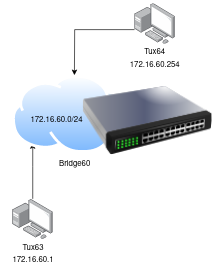
\includegraphics{experiment1}
Figure 1: Network configuration for experiment I
\subsubsection{Experiment Objectives}

This experiment had the purpose of teaching how to make 2 separate machines communicate over a network.

\subsubsection{Main Configuration Commands}

\begin{code-bash}
# tux3:
root# ifconfig eth1 up
root# ifconfig eth1 172.16.60.1/24

# tux4:
root# ifconfig eth0 up
root# ifconfig eth0 172.16.60.254/24

\end{code-bash}

In this experiment, the computers were connected to the switch with no additional configuration needed (thus using the switch's "default" bridge).

Note: due to a problem with the bench's tux3 ethernet sockets, tux3 had to use the \textit{eth1} interface and have the physical cable connected to the bench's \textit{E2} socket. This is the same for the remaining experiments.
\subsubsection{Log analysis}

The corresponding Wireshark log is included as an annex.

In tux3 we issued a ping command to \textit{172.16.60.254}. Since tux3 does not know the MAC address of the machine with this IP address (and as such does not know where to send the ping requests) it first makes an ARP request to resolve the MAC address corresponding to the pinged IP address.

ARP stands for Address Resolution Protocol, used by computers to associate an IP address with a MAC address in their respective "ARP tables", where all associations "IP Address - MAC Address" are stored for future use.

In this case, tux3 (MAC address \textit{00:22:64:a7:32:ab}) sends a "broadcast" ARP packet to discover who has IP address \textit{172.16.60.254}: this can be identified in the underlying Ethernet frame that includes the packet (the "destination" field is \textit{ff:ff:ff:ff:ff:ff}).
Upon receiving this broadcast packet, tux4 (MAC address \textit{00:21:5a:5a:75:bb}) sends a response to tux3 indicating that it has the IP address specified in the ARP request and returning its MAC address, which in turn is stored in tux3's "ARP table".

After getting tux4's MAC address, tux3 continuously sends PING requests and tux4 sends PING responses, each containing the previously mentioned MAC and IP addresses.

The type of packet sent in a frame can be differentiated using the 'type' field (bytes 13 and 14): IPv4 corresponds to type 0x0800, ARP corresponds to type 0x0806. ICMP packets are stored inside the IPv4 packet so they do not have a specific type code, even though the IPv4 packet itself has a field identifying the format of its data.
The length of each received frame can be calculated on a per-type basis:
\begin{itemize}
    \item IPv4 packets have a field named Total Length that represents the length of the IPv4 packet and its contents and is stored at bytes 3 and 4 of the packet header. So the total frame length is the packet's total length plus the length of the ethernet frame header.
    \item ARP packets themselves have a fixed length (in our experiments, and according to several online resources): always 28 bytes long. However, some padding can be added, making the frame length vary between 46 and 64 bytes (Wireshark omits the 4 CRC bytes included in the Ethernet frame and as such the lengths displayed vary between 42 and 60 bytes).
\end{itemize}

Besides the Ethernet interfaces present in both machines, there is also a "Loop-back" interface, which is a virtual network interface, in other words, it is implemented in software at the kernel level.
The primary purpose of this interface is to check the validity of the installed "network stack", which is necessary for every other type of network communication.
This is achieved by sending frames from a machine to itself: if either the frame's destination or source field is a loopback interface, the frame should not leave the current machine, instead being sent back up the network stack.
Other purposes include routing packets from a client (browser, for example) to a server running on the same machine (because the packets do not leave the current machine).

\subsection{Experiment II}

\subsubsection{Network Architecture}

At the end of the experiment, the network configuration should consist of tux63 and tux64 connected by a bridge (bridge0) and tux62 connected to a different bridge (bridge1) through the MicroTik switch, as follows:

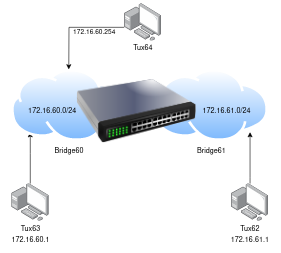
\includegraphics{experiment2}
Figure 2: Network configuration for experiment II

\subsubsection{Experiment Objectives}

The purpose of this experiment is to teach us how to setup 2 different network domains on the same switch, and verify that no communication occurs between these domains by default.

\subsubsection{Main Configuration Commands}

\begin{code-bash}
# These commands are performed after the configuration in experiment I

# tux2
root# ifconfig eth0 up
root# ifconfig eth0 172.16.61.1/24

# Switch, connected to through a serial cable
/system reset-configuration

/interface bridge add name=bridge60
/interface bridge add name=bridge61

# assuming tux2, tux3 and tux4 are connected to, respecitvely, switch sockets 10, 1 and 2:
/interface bridge port remove [find interface=ether1]
/interface bridge port remove [find interface=ether2]
/interface bridge port remove [find interface=ether10]
/interface bridge port add bridge=bridge60 interface=ether1
/interface bridge port add bridge=bridge60 interface=ether2
/interface bridge port add bridge=bridge61 interface=ether10
\end{code-bash}

\subsubsection{Log Analysis}

The corresponding Wireshark logs are included as annexes.

From the log analysis we can see that tux63 and tux64 can send and receive ping requests/responses from each other, since they are connected to the same bridge on the switch (bridge0).

However tux62 is still unreachable from the 2 other machines.
This hypothesis is backed by the capture logs taken from tux62: when pinging from tux63, both tux63 and tux64 show ICMP packets corresponding to PING requests/responses. However, tux62's logs never show any ICMP packets, indicating that this machine is not connected to either one of the other computers.
2The same thing happens when sending ping broadcasts from tux63 and tux62: tux63 is connected to tux64 and vice-versa, while tux62 is disconnected from the other two.

This also tells us that there are now 2 separate sub-networks operating through the switch. One way to confirm this is to verify the IP address in the 'sender' field in Ethernet frames sent from the 3 computers: tux64 and tux63 belong to the same network (172.16.60.0/24) while tux62 is connected to another network (172.16.61.0/24).

\subsection{Experiment III}

\subsubsection{Network Architecture}

At the end of the experiment, the network configuration should consist of tux63 and tux64 connected by a bridge (bridge0) and tux62 and tux64 connected by a different bridge (bridge1) through the MicroTik switch, as follows:

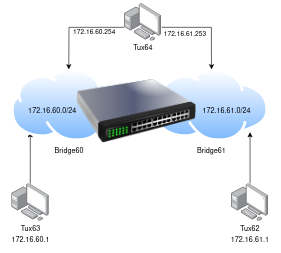
\includegraphics{experiment3}
Figure 3: Network configuration for experiment III

\subsubsection{Experiment Objectives}

The purpose of this experiment is to turn tux64 into a router in order to allow communication between tux63 and tux62.

\subsubsection{Main Configuration Commands}

\begin{code-bash}
# these commands are performed after the configuration in experiment II

# Switch
# these commands assume that tux64 is also wired to socket 11 of the switch
/interface bridge port remove [find interface=ether11]
/interface bridge port add bridge=bridge61 interface=ether11

# tux4
root# ifconfig eth1 up
root# ifconfig eth1 172.16.61.253/24
root# echo 1 > /proc/sys/net/ipv4/ip_forward
root# echo 0 > /proc/sys/net/ipv4/icmp_echo_ignore_broadcast

# tux3
root# route add -net 172.16.61.0/24 gw 172.16.60.254

# tux2
root# route add -net 172.16.60.0/24 gw 172.16.61.253
\end{code-bash}

\subsubsection{Log Analysis}

The corresponding Wireshark logs are included as annexes.

After connecting tux4 to both sub-networks and configuring routes through tux4 in both tux3 and tux2, these can send PING requests/replies to each other, as can be seen in tux3's logs. This confirms that the network configuration is correct.

If we inspect the routing tables in both tux3 and tux2 we can understand why this happens: tux4 (which is connected to both sub-networks) is the default gateway for both machines to access the sub-network they are not a part of.

After deleting the ARP tables in tux4 and re-running the ping command, the 3 tuxes do not know how to reach each other (since they do not know each other's MAC addresses).
Because of this, and because tux3 is pinging a machine on another network, tux3 sends an ARP broadcast to subnet 172.16.60.0/24 requesting the MAC address of its default gateway, in this case tux4.
An ARP response is generated and sent to tux3 which in turn stores the MAC address of tux4 in its ARP table for later use (later tux4 does the inverse process to store the MAC address of tux3).
Since the ping is going through tux4 into tux2, the same process happens in the second sub network, ending in tux4 storing the MAC addresses of both tux3 and tux2.

After that, routing of ICMP packets occurs normally. It should be noted that these packets have the source field set to the IP address of tux3 and destination field set to the IP address of tux2. However, the underlying frame's destination address (when the packet is sent by either tux3 or tux2) is set to tux4's MAC address.
This makes sense on a theoretical level since Ethernet frames are a Layer 2 data model and as such should be transmitted between connected nodes, where as IP packets are a layer 3 data model and store the transmission endpoints.
\subsection{Experiment IV}

\subsubsection{Network Architecture}

At the end of the experiment, the network configuration should consist of tux63 and tux64 connected through the MicroTik switch, as follows:

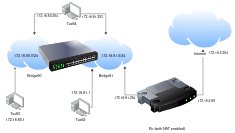
\includegraphics{experiment4}
Figure 4: Network configuration for experiment IV
\subsubsection{Experiment Objectives}

The purpose of this experiment is to add internet connectivity to the developed network through a commercial router connected to the labs network.

\subsubsection{Main Configuration Commands}

\begin{code-bash}
# these steps are performed after the ones described in experiment III    

# these steps assume that the router is connected to the switch on socket 12
# Switch
/interface bridge port remove [find interface=ether12]
/interface bridge port add bridge=bridge61 interface=ether12

# Router
/system reset-configuration
/ip address add address=172.16.2.69/24 interface=ether1
/ip address add address=172.16.61.254/24 interface=ether2
/ip route add dst-address=0.0.0.0/0 gateway=172.16.2.254
/ip route add dst-address=172.16.60.0/24 gateway=172.16.61.253

# tux4
root# route add default gw 172.16.61.254

# tux3
root# route add default gw 172.16.60.254

# tux2
# in the beginning of the experiment
root# route del default gw 172.16.61.254
# in the middle of the experiment
root# route add default gw 172.16.61.254

\end{code-bash}

\subsubsection{Log Analysis}

The corresponding Wireshark logs are included as annexes.

After deleting tux2's route through tux64, tux62 can only access the 172.16.60.0/24 sub-network through its default router, in this case the bench's router.
This can be confirmed by analyzing the capture logs taken from tux62: the IPv4 packets have the addresses of tux62 an tux63 but the Ethernet frames have different MAC addresses, belonging to the router and tux62.
Besides this, there were 2 ARP unicast requests made by tux62 and tux64 to resolve the MAC addresses of, respectively, the router and tux62.

All of this tells us that the ping request followed the following path: tux62 -> router -> tux64 -> tux63 -> tux64 -> tux62.

Afterwards, tux63 made pings to the labs router. These requests succeeded when NAT was enabled on the router and failed when it wasn't. This is due to the fact that the router was responsible for translating addresses outside the sub-networks to valid addresses on the sub-networks using NAT (Network Address Translation).

NAT is the mechanism through which a router machine (commercial router or not, in our case tux64 could be responsible for performing NAT if correctly configured) translates an incoming IP address into an outgoing IP address belonging to a sub-network. This can be used to avoid address collisions with external addresses (from a sub-network's "point of view").

\subsection{Experiment V}

\subsubsection{Network Architecture}

\subsubsection{Experiment Objectives}

\subsubsection{Main Configuration Commands}

\subsubsection{Log Analysis}

\subsection{Experiment VI}

\subsubsection{Network Architecture}

\subsubsection{Experiment Objectives}

\subsubsection{Main Configuration Commands}

\subsubsection{Log Analysis}

\section{Conclusions}

\onecolumn
\appendix
\section{Appendix}

\subsection{Code}

\noindent In folder \lstinline{src/}.

\end{document}
